\section{引言}

\begin{figure*}[tb]
    \centering
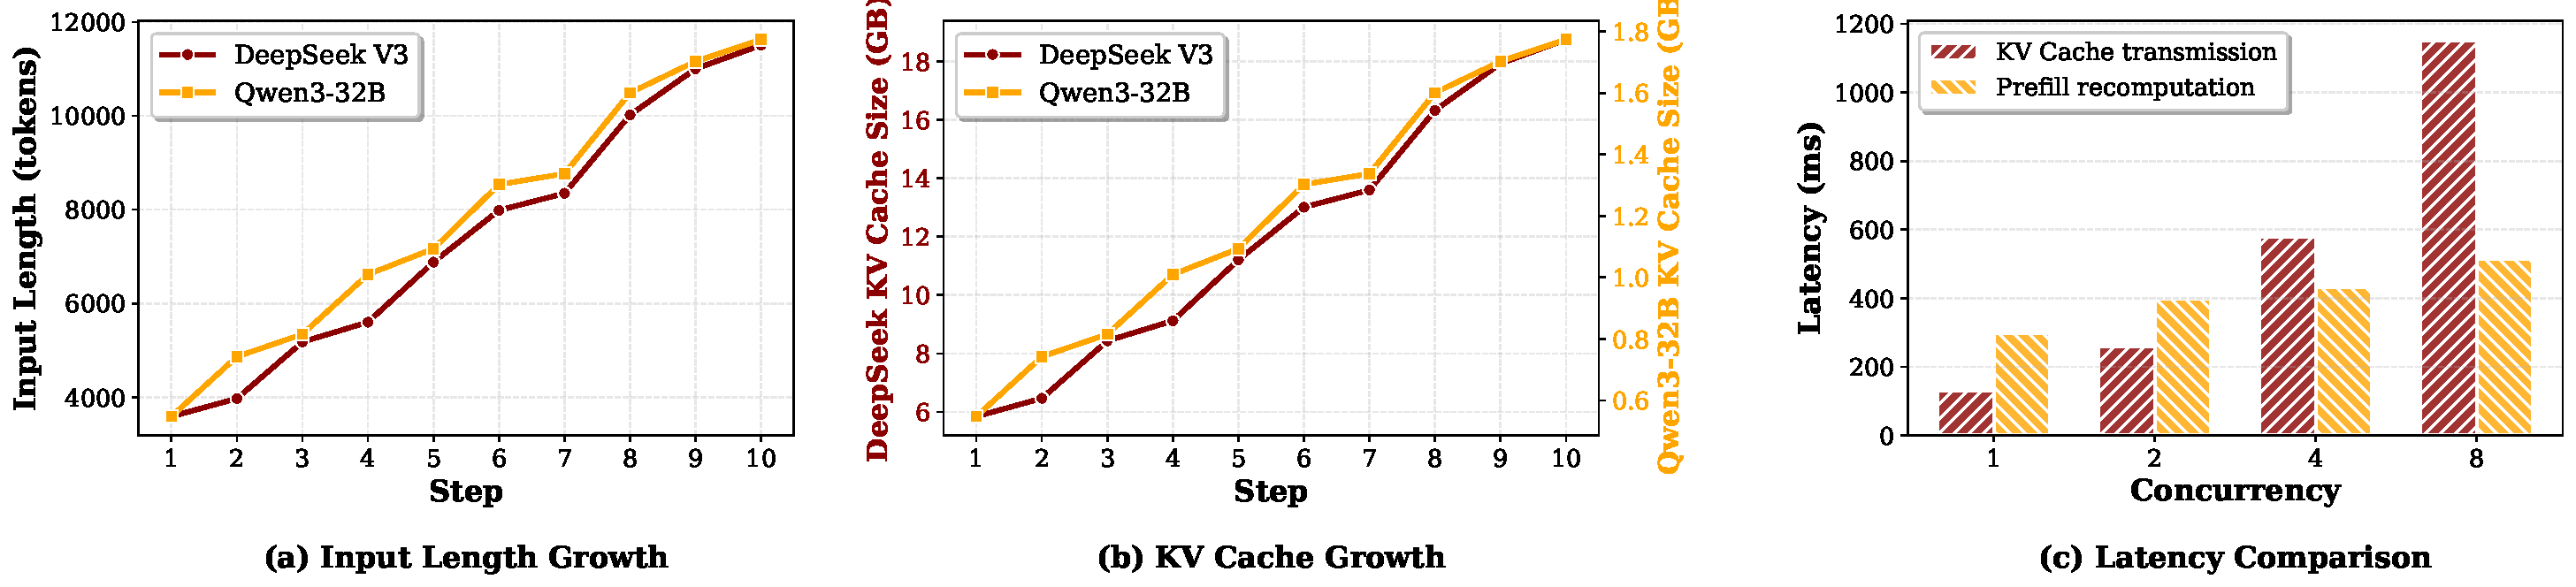
\includegraphics[width=0.98\linewidth]{figure/comprehensive_comparison.pdf}
    \caption{(a)(b) DeepSeek-V3 与 Qwen3-32B 在 10 个生成步内的输入长度与 KV 缓存显存占用增长情况。(c) 在不同并发度下，DeepSeek-V3（每个请求 6.67 GB 缓存、4096 token）的 GPU-CPU KV 缓存卸载时延与基于 prefill 的重计算时延对比。}
    \label{fig:comparisons}
\end{figure*}

大语言模型（LLM）正越来越多地以\emph{Agent} 的形式部署，在较长时间跨度内与外部环境交互 \cite{nex,rollpacker}。这使得高吞吐的 Agent 批量推理成为三类关键工作负载的计算基础设施：(1) Agent 强化学习 rollout，需要大规模并行轨迹生成以支撑策略优化，并占据端到端训练时间的主要部分 \cite{openrlhf,Laminar,respec}；(2) 数据蒸馏，即从高阶推理模型蒸馏数据，再用这些数据对学生模型进行监督微调 \cite{rl_distill}；(3) Agent 评测，其中模型需要并发地模拟并评估数千种不同场景 \cite{agentjudge}。

在 Agent 批量推理中，每个 Agent 的上下文都会随时间单调增长（见图~\ref{fig:comparisons}a），从而导致其 KV 缓存占用持续扩大（见图~\ref{fig:comparisons}b）。随着规模提升，驻留在 GPU 上的 KV 缓存不再只是一个静态加速结构，而会演变为一个高度竞争、不断变化的共享资源。

现代 LLM 服务引擎通常借助前缀缓存和淘汰机制来缓解 KV 缓存压力 \cite{chunkattention,hydragen,promptcache}。这些系统将缓存前缀组织为树结构 \cite{sglang}，并通过最近最少使用（LRU）策略淘汰节点，因此在具有高前缀重叠的聊天式工作负载上表现良好。当 GPU 显存不足时，被淘汰的 KV 缓存槽通常会被卸载到 CPU 内存，以 PCIe 传输时延换取更少的重计算 \cite{mooncake,preble,promptcache}。

然而，这些技术在 Agent 批量推理场景下会失效。核心问题不仅在于上下文变长，更在于\emph{Agent 的推进是异步的}。部分 Agent 正在主动生成 token，而另一些 Agent 则停在工具调用阶段，临时处于不活跃状态。采用标准 LRU 淘汰时，这些暂时不活跃但语义上仍然关键的前缀会在内存压力升高时被激进淘汰。等 Agent 恢复执行时，系统必须通过重计算或主机到设备传输来重建其完整前缀，而且这一代价会随着 Agent 已积累历史的增长而增加。图~\ref{fig:twoagent}a 在简化的三 Agent 场景中说明了这一失效模式。关键在于，即便系统中的 Agent 总数保持不变，这种额外开销也会被反复支付。

本文将这一病态行为识别并刻画为\emph{中期抖动（middle-phase thrashing）}。它不同于由简单容量耗尽导致的传统内存抖动，而是表现为执行中一段持续较长的低效时期。基于真实部署轨迹的分析（图~\ref{fig:dpskthrashing}a）表明，Agent 批量推理具有鲜明的三阶段执行模式。系统先经历一个短暂的预热阶段，缓存效率逐步提升；随后进入中期阶段，此时 GPU 显存仍处于饱和附近，但缓存命中率却显著塌陷。在这个阶段，系统陷入淘汰与重计算的恶性循环，导致吞吐显著下降。反直觉的是，即使模型规模与硬件资源不变，在这一阶段继续增加 Agent 数量反而会降低整体吞吐。

为应对这一挑战，我们认为 Agent 批量推理需要从被动缓存管理转向\emph{主动的 Agent 级准入控制}。我们的灵感来自分布式系统中的拥塞控制 \cite{congestion_control,chiu1989analysis,tcp}：访问有限共享资源时，系统依赖反馈驱动的控制环来避免资源过载。沿着这一思路，我们将 GPU 上的 KV 缓存视为一种共享且有限的资源，并提出 \SysName{}。它不是替换现有服务栈，而是在 Agent 执行框架与现有 LLM serving engine 之间插入一个轻量级控制层，基于缓存使用率与命中率等运行时信号动态调节活跃 Agent 的数量，从而在维持较高利用率的同时避免中期抖动。

本文的主要贡献如下：
\begin{itemize}[leftmargin=*,nosep]
    \item 我们识别并系统刻画了 Agent 批量推理中的中期抖动现象，说明其根源在于异步 Agent 推进、持续增长的上下文，以及请求级被动淘汰策略之间的失配。
    \item 我们提出 \SysName{}，将拥塞控制思想引入 Agent 推理，通过 Agent 级准入控制限制总体 KV 工作集规模，并保持执行连续性。
    \item 我们在真实 Agent 工作负载与大模型上验证了该方法的有效性。\SysName{} 在 Qwen3-32B 上可带来最高 $4.09\times$ 的吞吐提升，在 DeepSeek-V3 上可带来最高 $1.90\times$ 的提升，同时与现有 LLM 服务系统兼容。
\end{itemize}
